\chapter{Monotonic Capacitor Switching DAC}


\textit{\textbf{Abstract:} This chapter presents details of building blocks of D to A converter, which is used in proposed A to D converter, that uses a monotonic capacitor switching procedure. The fundamental building blocks are the comparator, capacitor network and bootstrapped switch.} 


\section{Bootstrapped switch}

\par
\hspace{1.2cm} The bootstrapped switch~\cite{760369} shown in Fig.~\ref{fig:BSS} performs the track and hold function. With the bootstrapped switch, the gate-source voltage of the sampling transistor is fixed at the supply voltage, which makes the on-resistance a small constant value and thus improves the switch linearity.

\begin{figure}[ht]
	\begin{center}
		\includegraphics[scale=0.4]{./Figures/BootstapSwitch.eps}
		\caption{Circuit Diagram of Bootstrapped switch}
		\label{fig:BSS}
	\end{center}
\end{figure}


\section{Dynamic Comparator}

\par
\hspace{1.2cm} Fig.~\ref{fig:CTC} shows a schematic of the dynamic comparator. During the conversion phase, the $Clk$ input to the voltages comparator approach ground, the comparator uses a p-type input pair. Because a dynamic comparator does not consume static current, it is suitable for energy efficient design. When $Clk$ is high, the comparator output $V_{out}$ is reset to zero. When $Clk$ goes to low, the differential pair, $M_{3}$ and $M_{4}$, compares the two input voltages. Then, the latch regeneration forces one output to high or low depending up on the values of analog input signals. 

\begin{figure}[ht]
	\begin{center}
		\includegraphics[scale=0.45]{./Figures/CTComparator.eps}
		\caption{Circuit Diagram of Dynamic Comparator}
		\label{fig:CTC}
	\end{center}
\end{figure}


\section{Monotonic Switching Procedure}

\par
\hspace{1.2cm} In conventional A to D converters at the sampling phase, the bottom plates of the capacitors are charged to $V_{ip}$ and the top plates are reset to the common-mode voltage $V_{cm}$. Next, the largest capacitor $C_{1}$ is switched to $V_{ref}$ and  the other capacitors are switched to ground. The comparator then performs the first comparison. If $V_{ip}$ is higher than $V_{in}$ , the most significant bit (MSB) $B_{1}$ is set to 1. Otherwise, $B_{1}$ is set to 0, and the largest capacitor is reconnected to ground. Then, the second largest capacitor $C_{2}$ is switched to $V_{ref}$. The comparator does the comparison again. This procedure repeats until the least significant bit (LSB) is decided. Although the trial and error search procedure is simple and intuitive, it is not an energy efficient switching scheme~\cite{5437496}, especially when unsuccessful trials occur. Fig.~\ref{fig:CADC} shows the conventional SAR A to D converter.

\begin{figure}[ht]
	\begin{center}
		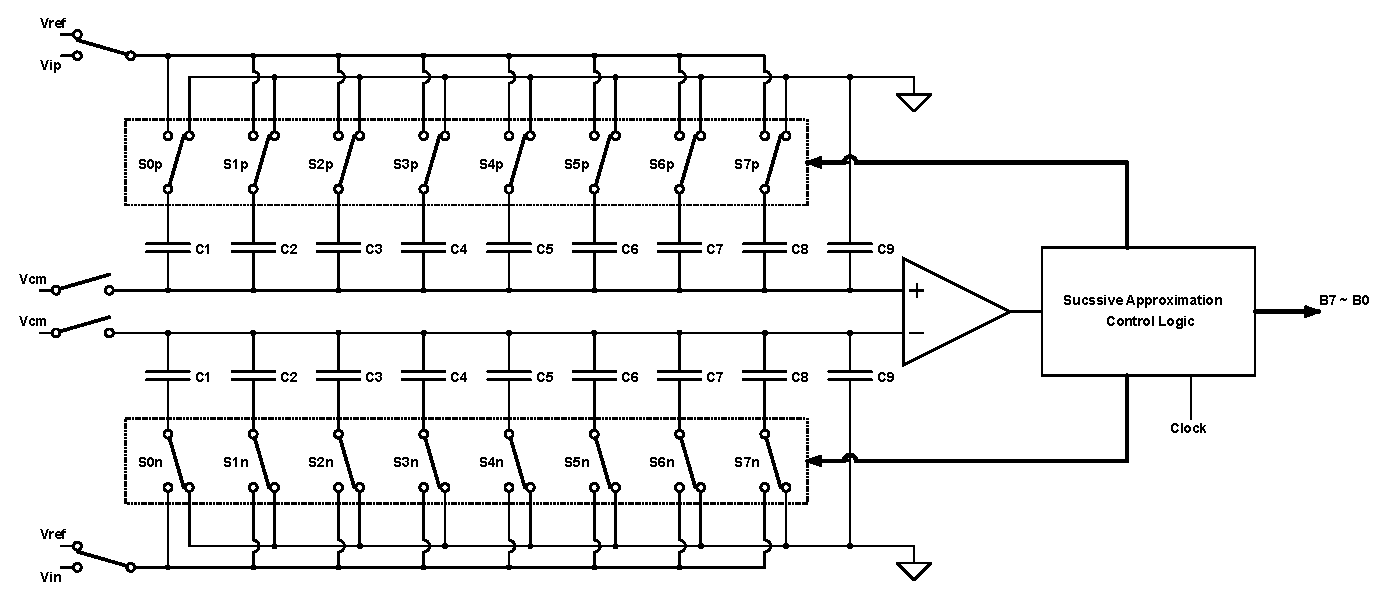
\includegraphics[scale=0.68]{./Figures/ConventionalDAC.eps}
		\caption{Block Diagram of Conventional SAR ADC}
		\label{fig:CADC}
	\end{center}
\end{figure}

\par
\hspace{1.2cm} Fig.~\ref{fig:MADC} shows the monotonic capacitor switching SAR A to D converter~\cite{5437496}, where the monotonic switching can be either upward or downward. This A to D converter samples the input signal on the top plates via bootstrapped switches. At the same time, the bottom plates of the capacitors are set to $V_{ref}$. Next, after the A to D converter turns off the bootstrapped switches, the comparator directly performs the first comparison without switching any capacitor. According to the comparator output, the largest capacitor $C_{1}$ is connected to ground or kept at $V_{ref}$. The A to D converter repeats the procedure until the LSB is decided. For each bit cycle, there is only one capacitor switch, which reduces both charge transfer in the capacitive D to A converter network and the transitions of the control circuit and switch buffer, resulting in smaller power dissipation. 


\begin{figure}[ht]
	\begin{center}
		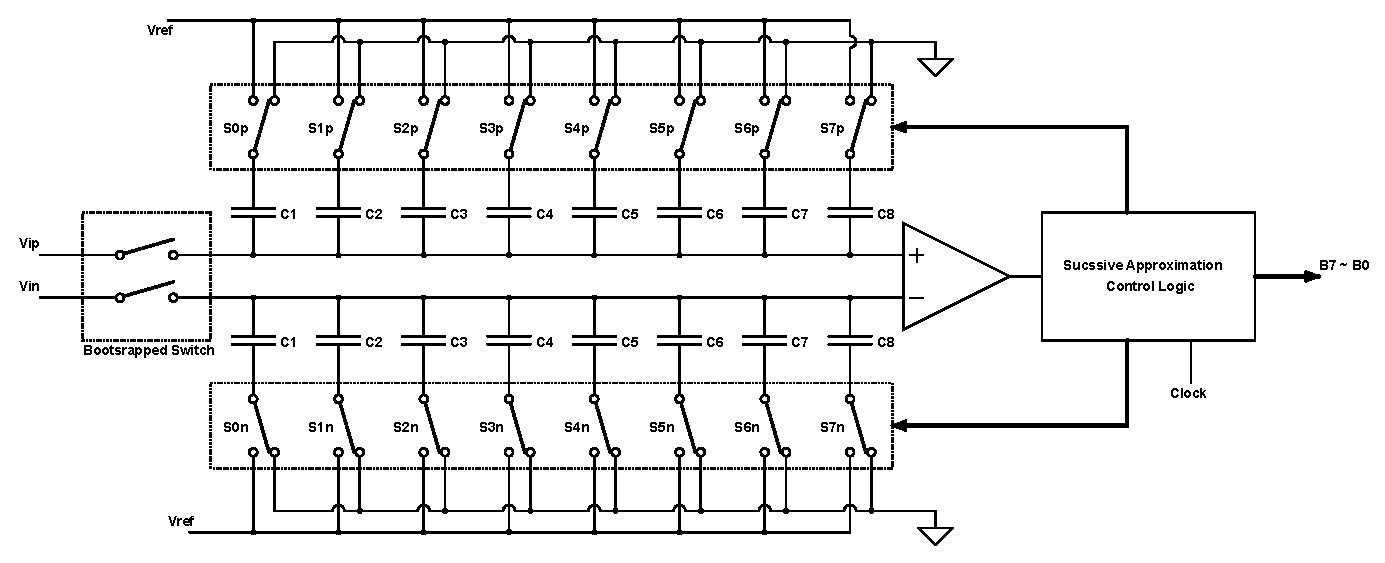
\includegraphics[scale=0.68]{./Figures/WorkingDAC.eps}
		\caption{Block Diagram of Monotonic Capacitor Switching ADC}
		\label{fig:MADC}
	\end{center}
\end{figure}



\par
\hspace{1.2cm} One of the major differences between the monotonic capacitor switching SAR A to D converter method and the conventional one is that the common-mode voltage of the reference D to A converter gradually decreases from half $V_{ref}$ to ground. The monotonic switching sequence does not require upward transition. In addition, since sampling is done on the top plate, the comparator can do the first comparison without any capacitor switching. For an n-bit A to D converter, the number of unit capacitors in a capacitor array is $2^{n-1}$, only half that of the conventional one. Fig.~\ref{fig:CSP} shows 3-bit examples of the conventional and monotonic capacitor switching methods.

\begin{figure}[ht]
	\begin{center}
		\subfloat[Conventional switching procedure]{\label{fig:CSM}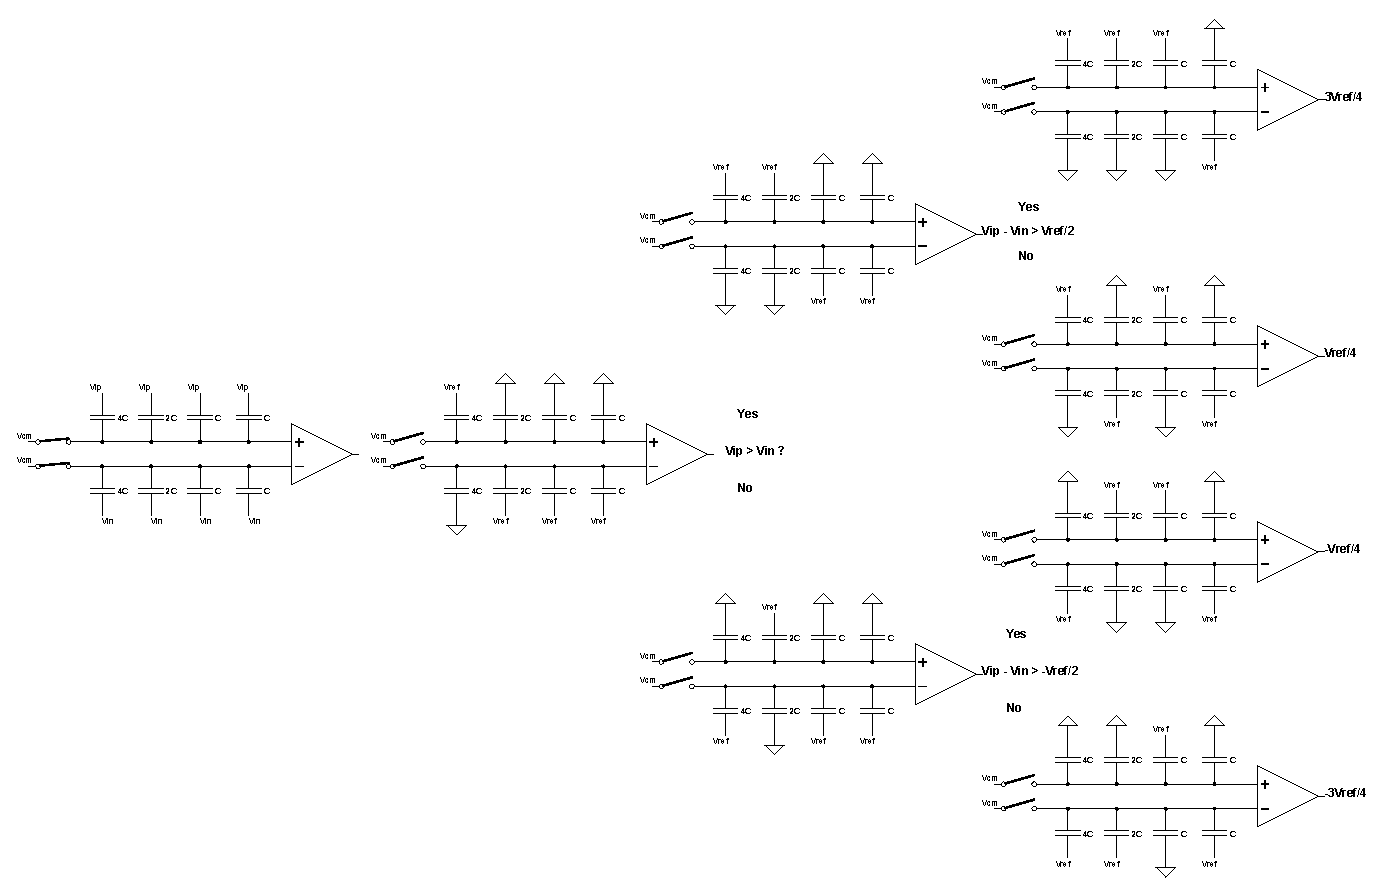
\includegraphics[scale=0.504]{./Figures/ConventionalSwitching.eps}} \\
		\subfloat[Monotonic Switching  procedure]{\label{fig:MSM}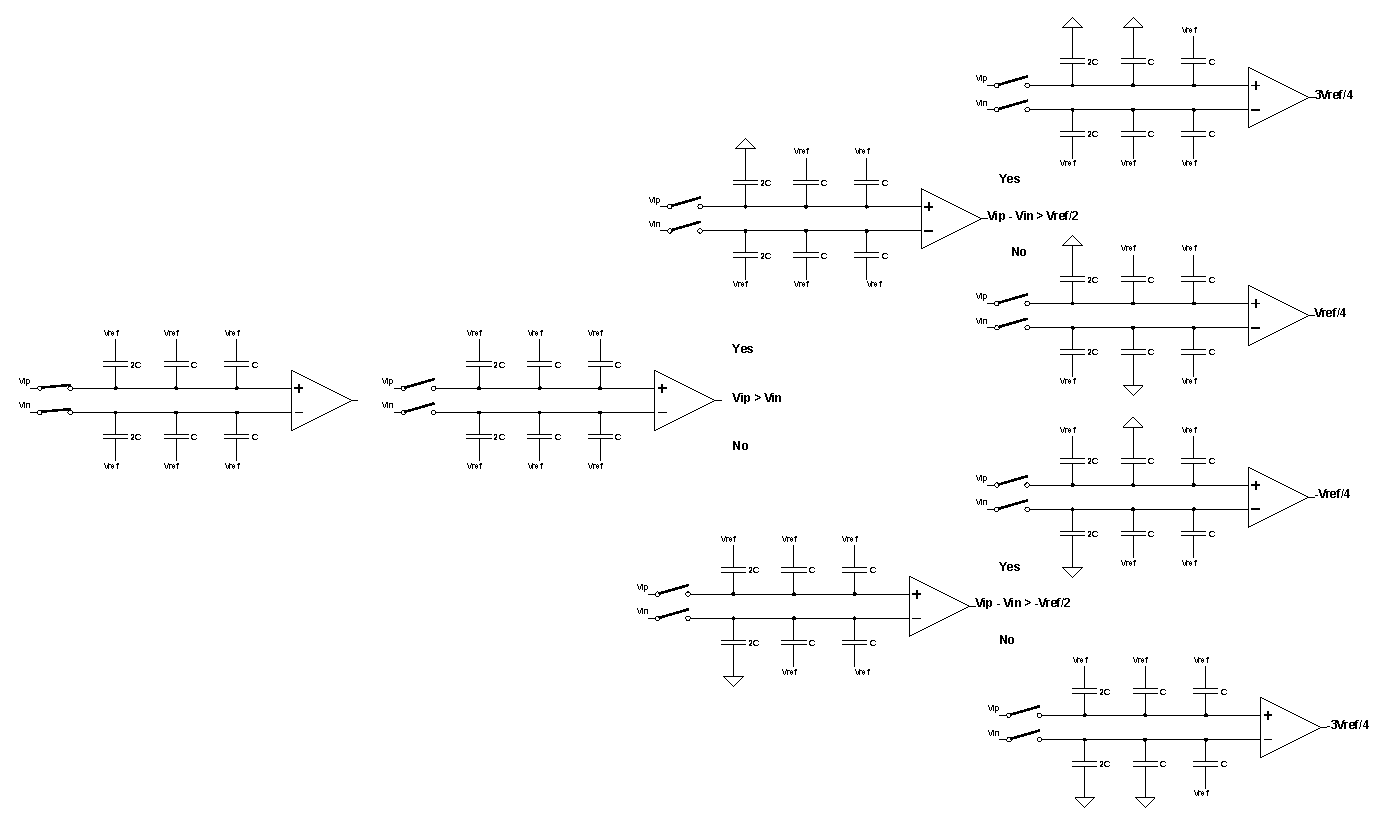
\includegraphics[scale=0.504]{./Figures/MonotonicSwitching.eps}}
		\caption{Capacitor Switching procedure}
		\label{fig:CSP}
	\end{center}
\end{figure}

\par
\hspace{1.2cm} The conventional switching method is based on a trial and error search procedure. Fig.~\ref{fig:CSM} shows all possible conversions in a 3-bit conventional switching method. The conventional switching sequence is efficient when all the attempts are successful, as in the upper cases. However, the switching sequence consumes a lot of energy when attempts are unsuccessful, as in the lower cases. Fig.~\ref{fig:MSM} shows all possible switching cases of the monotonic capacitor switching method. After the sampling switches turn off, the comparator directly performs the first comparison without switching any capacitor. Therefore, the monotonic switching sequence consumes no energy before the first comparison. In contrast, the conventional sequence consumes $4CV^2_{ref}$ before the first comparison.



\begin{figure}[ht]
	\begin{center}
		\includegraphics[scale=0.45]{./Figures/MixedSignalDesignFlow.ps}
		\caption{Design Flow for proposed A to D Converter}
		\label{fig:MDF}
	\end{center}
\end{figure}











